%%%
%%% Introduction.
%%%

\svnInfo $Id$

\newcommand\schema[1]{\ensuremath{\mathcal{#1}}}
\newcommand\relation[1]{\ensuremath{\textnormal{\bf\textsf{#1}}}}

\makeatletter
\newcommand\skyline{\mathop{\operator@font skyline}\nolimits}
\newcommand\skyband{\mathop{\operator@font skyband}\nolimits}
\makeatother

\newcommand\imp{\Rightarrow}
\newcommand\bigland{\bigwedge}
\newcommand\biglor{\bigvee}
\newcommand\union{\cup}
\newcommand\bigunion{\bigcup}
\newcommand\intersection{\cap}
\newcommand\difference{\backslash}
\newcommand\dominates{\ensuremath{\succ}\xspace}
\newcommand\weakdominates{\ensuremath{\succeq}\xspace}

\newcommand\inlinesql[1]{{\tt #1}}
\newcommand\srcref[1]{{\tt #1}}
\newcommand\postgresdocu[2]{\href{http://www.postgresql.org/docs/8.3/static/#1}{#2}\footnote{\url{http://www.postgresql.org/docs/8.3/static/#1}}}
\newcommand\ttbackslash{{\char92}}

\newtheorem{definition}{Definition}
\newtheorem{lemma}{Lemma}
\newtheorem{theorem}{Theorem}


\makeatletter
\newenvironment{shellscript}
{\begingroup\list{}{\listparindent 0\p@\itemindent\listparindent\leftmargin15\p@\rightmargin15\p@}\item[]\begin{alltt}}{\end{alltt}\endlist\endgroup}
\makeatother

\newcommand\cmd[1]{\textcolor{blue}{> #1}} \fixme{}{fix command prompt}

\section{TODO}
\begin{itemize}
\item \todo{casing of section headings?}{}
\item \todo{ask ali, which website for travelling by airplane uses skyline}{}
\item \todo{using hashing for diff groups}{}
\item \todo{EF+SFS=LESS (check this again)}{}
\item \todo{has the order in which the skyline dimensions are checked an effect?}{}
\item \todo{show how Preference SQL ABOUT can be emulated}{}
\item \todo{PostgreSQL as of 8.3 does not derive the stats for subselect like \inlinesql{explain analyze select * from (select * from i15d1000000s0 limit 1000) as a skyline of d1 min, d2 min with windowpolicy=ranked;}}{}
\end{itemize}
\clearpage


\chapter{Introduction\revision}
\label{chap:Introduction}

\section{General Introduction}
\todo{}{take some parts from the research planning intro}

give the intuition.

\subsection{motivation}
motivation: green computing: less cpu time, less computers, less energy --> safe the planet

stocks: risk vs. costs (--> streaming skyline see [Tao2006])

example of skyline

when travelling by airplane: time vs. costs

TODO: more dim: \#stops, total dist
travel by bus: \#of visited cities

it is shown on some website. which?

Credit To: Ali (room mate)

employee (salary, revenue, years in the company)

\subsection{consider only bnl and sfs}

from \citep{Chaudhuri2006}:

In this paper, our focus is on algorithms that can be
directly implemented in today's commercial database systems
without the addition of new access methods (which
would require addressing the associated challenges of maintenance
with updates, concurrency control, etc.). Specifically,
we consider the Block-nested-loop Algorithm [15],
and the Block-nested-loop with Presorting [5].

Special algorithms have been proposed for the case the whole relation fits into main memory \citep{Preparata1985}, nevertheless we do not take them into account as memory is always a short resource in a database scenario, either due to the number of concurrent users or limited total main memory, e.g. on a handheld device.

The skyline operator \citep{Borzsonyi2001} filters out the \emph{interesting} points from a potentially large set of data points. The skyline operator returns the pareto optimal\index{pareto optimal} elements of a set. This is also know as maximum vector problem\index{maximum vector problem}.

\section{Related Problems}
Convex hull, \emph{top-K} queries, and nearest-neighbor search (especially in the context of spacial skylines ``give me the next good restaurant'')

In particlar, the convex hull contains the subset of skyline points that may be optimal only for linear preference functions (as opposed to any monotone function).\todo{from \citep{Papadias2005}}{rephrase}





\clearpage 
\fixme{}{no clearpage}
\section{Basic definitions}
\todo{We are in the context of relational model\index{relational model} of data}{\citep{Chomicki2002, Chomicki2003a}?}. As we aim at an implementation of the skyline operator into a relational database management system (RDBMS)\index{RDBMS} we restrict to finite database\index{finite database} instances.

We assume two \todo{infinite}{hm? although in a real computer is everything finte} domains: $N$ (numbers) and $D$ (uninterpreted constants). The domain $D$ will be used for attributes which are not subject to skyline computation, i.e. for the travelling example we will not use the name of the airline as a skyline criterion, therefore $D$ will be used as domain for this attribute.
For attributes or expressions which are subject to skyline computation we use the domain $N$. No distinction is made between different numeric domains, since it is not necessary for this paper. For $N$ we require that equality ($=$), inequality ($\not=$), and the binary relations $<$ (strictly less than), $\le$ (less than or equal), $\ge$ (greater than or equal), and $>$ (strictly greater than) are defined with the usual properties.

\begin{definition}[Schema]
Given the domains $U_i, 1 \le i \le n$, such that $U_i$ is either equal to $D$ or $N$, we define the $n$-ary schema $\schema{R}$ as the cartesian product of the $U_i$'s, i.e. $\schema{R} = U_1 \times U_2 \times \ldots \times U_n$. The attributes of schema \schema{R} will be refered as $a_1, \ldots, a_n$.
\end{definition}

Preferences will be defined in terms of \emph{binary preference relations}\index{preference relation}.
\begin{definition}[Preference relation]
Let \schema{R} be a $n$-ary schema, a relation \dominates is a preference relation over \schema{R} if it is a subset of $\schema{R} \times \schema{R}$.
\end{definition}

To give an intuition, \dominates will be a binary relation between pairs of tuples from the same (database) relation, we say $r$ \emph{dominates} $s$ in \dominates iff $(r, s) \in \dominates$ (or in infix notation $r \dominates s$).

We require the relation \dominates to be a \emph{strict partial order}\index{strict partial order}, i.e. \dominates is irreflexive, asymmetric and transitive. These properties are formalized as usual:

\begin{itemize}
\item \emph{irreflexivity:} $\forall x: x \not\dominates x$
\item \emph{asymmetry:} $\forall x, y: x \dominates y \imp y \not\dominates x$
\item \emph{transitivity:} $\forall x, y, z: (x \dominates y \land y \dominates z) \imp x \dominates z$
\end{itemize}

Non-transitive\index{non-transitive} preferences can be compute with the \todo{Best}{special font for algo names?} algorithm (\citep{Torlone2002, Ciaccia2004}), we will not study this approach in this paper.

\begin{definition}
\todo{}{}Let \relation{R} be a relation of schema \schema{R}.
\end{definition}

\begin{definition}[Skyline]
The skyline of a relation \relation{R} with respect to the preference relation \dominates is the set of tuples $r \in \relation{R}$ which are not dominate by any other tuple $s \in \relation{R}$, formally $\skyline_\dominates(\relation{R}) := \{ r \in \relation{R} | \nexists s \in \relation{R} : s \dominates r \}$
\end{definition}

\begin{lemma}
\todo{}{this is more or less theorem 2 from \citep{Chomicki2002}}
Given the relation $\relation{R} \not= \emptyset$ and \dominates a strict parial order over \schema{R}, where \schema{R} is the schema for \relation{R}, the skyline is non empty, i.e. $\skyline_\dominates(\relation{R}) \not= \emptyset$ holds.
\end{lemma}


In a skyline query with the following skyline clause:
\todo{}{add space between dim and direction}
\[
\texttt{SKYLINE OF} a_1 \texttt{MIN}, \ldots, a_k \texttt{MIN}, a_{k+1} \texttt{MAX}, \ldots, a_l \texttt{MAX}, a_{l+1} \texttt{DIFF}, \ldots, a_m \texttt{DIFF}
\]
a tuple 
$r = (r_1, \ldots, r_k, r_{k+1}, \ldots, r_l, r_{l+1}, \ldots, r_m, r_{m+1}, \ldots, r_n)$
dominates a tuple
$s = (r_1, \ldots, r_k, r_{k+1}, \ldots, r_l, r_{l+1}, \ldots, r_m, r_{m+1}, \ldots, r_n)$
iff the following condition holds
\begin{eqnarray}\label{equ:skylinepf}
\left( \bigland_{1 \le i \le k} r_i \le s_i \right) \land
\left( \bigland_{k+1 \le i \le l} r_i \ge s_i \right) \land
\left( \bigland_{l+1 \le i \le m} r_i = s_i \right) \land \nonumber\\
\land
\left( \left( \biglor_{1 \le i \le k} r_i < s_i \right) \lor
       \left( \biglor_{k+1 \le i \le l} r_i > s_i \right) \right).
\end{eqnarray}

To state in an informal way, a tuple $r$ dominates a tuple $s$ if it is equal in all \inlinesql{DIFF} dimensions, at least as good in all \inlinesql{MIN}/\inlinesql{MAX} dimensions and better than in at least one of the \inlinesql{MIN}/\inlinesql{MAX} dimensions.

\todo{make \dominates equal to (\ref{equ:skylinepf}) and \weakdominates equal to just the $\le$ part, use $r \sim s := r \weakdominates s \land s \weakdominates r = \forall i \in \{1, \ldots, m\}: r_i = s_i$, i.e. equal on all skyline dimensions}{}


If $\forall i \in \{1, \ldots, m\}: r_i = s_i$ holds, $r$ and $s$ are \todo{\emph{incomparable}}{use an other term for this special case of incomparability}, if \inlinesql{DISTINCT} is specified it is left up to the implementation to include either $r$ or $s$ in the skyline, if \inlinesql{DISTINCT} is not specified $r$ and $s$ are included. 


In case condition (\ref{equ:skylinepf}) does not hold $r$ and $s$ are \emph{incomparable} and may both be part of the skyline if not dominated by any other tuple from \relation{R}.

Please note that the following subformula (\ref{equ:skylinepfdiff}) of formula (\ref{equ:skylinepf}) induces an equality relation on \relation{R}, i.e. \relation{R} is partitioned into groups where the attributes $a_{l+1}, \ldots, a_m$ are equal:
\begin{equation}\label{equ:skylinepfdiff}
\bigland_{l+1 \le i \le m} r_i = s_i.
\end{equation}

\todo{As noted in \citep{Chomicki2003}, the \inlinesql{DIFF} directive works as a group by within the skyline, and the skyline for each group of diff attributes' values is found.}{rephrase}

This property can be exploited, if an ordered index on any subset of the attributes $a_{l+1}, \ldots, a_m$ exists, since the tuple window can be flushed each time the group is changed.

\todo{or in SFS due to the sort phase}{}, \todo{give an example with an table}{}

\subsection{Skyline as special case of winnow}
The skyline operator is a special case of the \emph{winnow operator}\index{winnow operator} \citep{Chomicki2002}, where the preference formula has exactly the form of formula (\ref{equ:skylinepf}).

Since the preference relation induced by the skyline criteria is a strict partial order, the following theorem (a special case of a theorem in \citep{Chomicki2002}) holds:

\begin{theorem}\label{theorem:nonempty}
For every finite, nonempty instance \relation{R} of \schema{R}, $\skyline_C(\relation{R})$ is nonempty.
\end{theorem}
\todo{}{the criteria C must be clearly defined}
If the relation \relation{R} fails to be finite, it may happen that $\skyline_C(\relation{R}) = \emptyset$, for example if \relation{R} contains all natural numbers and the standard ordering $<$ is used.


\begin{lemma}
Let $\relation{S} = \skyline_C(\relation{R})$, it is clear that condition (\ref{equ:skylinepf}) does not for any two tuples in \relation{S}.
\end{lemma}


\subsection{Further notions}
dominance, anti dominance region

\subsection{How our implementation differs from the mathematical model}
Our implementation of the \inlinesql{SKYLINE OF} clause is actually a bit more flexible than the mathematical definition given above. With our implementation the skyline operator is not restricted to attributes with a numerical domain, it can be applied to any attribute, as long as a \emph{sort function} is defined for the domain in question, i.e.\/ any expression valid in a SQL \inlinesql{ORDER BY} clause is valid as an expression in a \inlinesql{SKYLINE OF} clause.

This gives the opportunity to include expressions of almost any data type in a skyline query, even user defined ones, since it is possible to user define fullfledged data types in PostgreSQL. For more information on user defined data types see PostgreSQL documentation on \postgresdocu{xtypes.html}{User-Defined Types} and \postgresdocu{xindex.html\#XINDEX-OPFAMILY}{Operator Classes and Operator Families}

Anyway it is somewhat questionable what it is good for the include a e.g. \inlinesql{VARCHAR} column in a skyline query, still it is possible.

Furthermore our implementation allows arbitrary expressions instead of a single attribute, e.g.

\begin{sql}
SELECT * FROM nba.players \\
SKYLINE OF (h\_feet * 12 + h\_inches) MAX NULLS LAST, weight MAX NULLS LAST
\end{sql}

\subsection{Skyline Operator is Idempotent}
We first proof a more general statement:
\begin{theorem}\label{the:skyline-idempotent}
The winnow operator is idempotent, i.e. $\omega_C(\relation R)=\omega_C(\omega_C(\relation R))$.
\end{theorem}
\begin{proof}
\todo{no na}{}
Let $\succ$ be the preference relation induced by $C$, then the result of the winnow operator is $\omega_C(\relation R) := \{r \in \relation R | \nexists s \in \relation{R} : s \succ r \}$, so $\omega_C(\relation R)$ already contains only the maximal elements according $\succ$, \todo{...}{complete}
\end{proof}
Since the skyline operator is a special case of \emph{winnow} operator, theorem \ref{the:skyline-idempotent} holds as well.

\subsection{Composition of Skyline Operator}
\todo{For means of simplicity we assume set semantics?}{} \todo{The proofs are for the non \inlinesql{SKYLINE OF DISTINCT} case}{?}.


In this section, we study serveral ways of composing the skyline operator. (see \citep{Chomicki2002} 4.1)
We assume two finite instances \relation{R}, \relation{S} of schema \schema{R}, ...

\begin{equation}
\skyline(\relation{R} \intersection \relation{S}) = \skyline(\relation{R}) \intersection \skyline(\relation{S})
\end{equation}

this identity could be exploitet in the query optimizer. \todo{}{further work?}
is it really worth? what direction of the identity is actually iteresseting?

\begin{equation}\label{equ:skyline-composition-union}
\skyline(\relation{R} \union \relation{S}) \not= \skyline(\relation{R}) \union \skyline(\relation{S})
\end{equation}
It is easy to see that an equality in (\ref{equ:skyline-composition-union}) would not hold, as e.g. a single tuple $r_1$ could dominate the entire relation \relation{S}.

If the last property would hold, easy decompose, but due to theorem (\ref{theorem:nonempty}) $skyline(\{t_1\}) = \{t_1\}$ would yield $\forall \relation{R} : \skyline(\relation{R}) = \relation{R}$ if decompossied to singletons.

\begin{equation}\label{equ:skyline-decompose}
\skyline(\relation{R} \union \relation{S}) = \skyline(\skyline(\relation R) \union \skyline(\relation S))
\end{equation}
\begin{proof}
\todo{copy proof from manuscript}{}
\end{proof}

This property could be of interest in a distributed setting to reduce data transfer between servers.


\begin{equation}
\skyline(\relation{R} \difference \relation{S}) \not= \skyline(\relation{R}) \difference \skyline(\relation{S})
\end{equation}

\todo{}{make this plausible}

\todo{transitive closure}{4.2}
well all skyline query are transitive, so there is no need to investigate this here. But e.g. I prefer to eat Tafelspitz than to eat Schnitzel, and Schnitzel over Foobar. Thus, I also prefer to eat Tafelspitz than to eat Foobar.

\todo{skyline and joins, cross products, selections, projects, top k}{}

$\sigma_{Price<\textnormal{\euro}20}(\skyline_{C_1}(\relation{R}))=\skyline_{C_1}(\sigma_{Price<\textnormal{\euro}20}(\relation{R}))$
according to Theorem 3 (\citep{Chomicki2002}).
Such identies are not in our implementation.\todo{}{further work}

NOTE: $\sigma_{Price>\textnormal{\euro}20}$ does not commute with $\skyline$.


\texttt{TOP $k$} are realized with \inlinesql{LIMIT}

\subsection{Preference hierarchies}
(see 4.3 \citep{Chomicki2002}) ... I generally prefer red wine, but for fish I prefer white wine.
\todo{}{I think this can not be formulated using skyline}


\subsection{Intrinsic vs. extrinsic}
According to the defintion in 5.2 \citep{Chomicki2002} the skyline operator is \emph{intrinsic} as the preference relation between two tuples purles on the basis of the values occurring in those tuples. \todo{In contrast \emph{extrinsic} preference formulas may refer not noly to build-in predicats but also to other constructs, e.g., database relations.}{rephrase or cite}.

\subsection{Skyline Stratum and $K$-Skyband}
\todo{draw a nice diagram}{}

In the context of \emph{winnow} operator this is references as \emph{ranking}\index{ranking}, we prefer to use the term \emph{stratum}\index{stratum}, as we reserve the term ranking for scoring functions (see \ref{subsec:scoring}).

The $n$th skyline startum $\skyline_C^n$ is recursifly defined as:

\begin{eqnarray}
\skyline_C^1(\relation{R}) & := & \skyline_C(\relation{R}) \\
\skyline_C^{n+1}(\relation{R}) & := & \skyline_C(\relation{R} \difference \bigunion_{1 \le i \le n} \skyline_C^i(\relation{R}))
\end{eqnarray}

To give an example, the query $\skyline_C^2(\relation{R})$ computes the set of ``second-best'' tuples.\todo{}{rephrase or cite}

The startum are of interesset especially if there is a single or very few dominating tuples. In the context of the relation \emph{Hotel(Price, Distance to beach)}, a hut on the beach might be cheaper and closer to the beach than any other \todo{Unterkunft}{translate}, but might to meet our standards. \todo{restaurat, close, good, tiered of eating there}{}

A \emph{$K$-skyband}\index{$K$-skyband} query, introduced by \citet{Papadias2005}, is a simlar concept as skyline stratum. A $K$-skyband query reports all tuples which are dominated by at most $K$ points.

\fixme{It is easy to see, that the following identities hold}{thats wrong}
        x3
  x1  
 
    x2

x1, x2 are in stratum 1, x3 is in stratum 1 but while x1 and x2 are in 0-skyband, x3 is not is 1-skyband because it is dominiated by x1 and x2 so it is in 2-skyband. Hence no general relation can be established between K-skyband and skyline stratum.

The skyband rank of a point $p$ can be computed by counting the points in the anti-dominace region of $p$.

\begin{eqnarray}
\skyband_C^0(\relation{R}) &=& \skyline_C^1(\relation{R}) \label{equ:skyband} \\
\skyband_C^n(\relation{R}) &\not=& \bigunion_{1 \le i \le n+1} \skyline_C^i(\relation{R}) \quad \textnormal{for}\ n \ge 0\label{equ:skybandgeneral} \\
\skyline_C^n(\relation{R}) &\not=& \skyband_C^{n+1}(\relation{R}) \difference \skyband_C^n(\relation{R}) \quad \textnormal{for}\ n \ge 1
\end{eqnarray}

The branch-and-bound-skyline (BBS) \citep{Papadias2005} supports the computation of $K$-skyband queries, as stated by \citet{Papadias2005}, BNL and SFS can compute $K$-skybands, this can be easly done by maintaining a the number of tuples that dominate a tuple in the tuple window. Increase the number by one each time a tuple in the tuple window is dominated by the current tuple and once this count is greater than $K$ drop the tuple from the tuple window.


An interessing combination of \inlinesql{SKYLINE OF} and \inlinesql{TOP $k$} is given by the \emph{top-$k$-skyline}\index{top-k-skyline} operator \todo{\citep{Brando2007, Goncalves2005a, Goncalves2005}}{check citation}, where as many skyline startum are computed till at least $k$ tuples are found, or the entire relation is returned.


\subsection{Monoton vs. linear scoring functions}\label{subsec:scoring}
see \citep{Chomicki2002a} page 5, Theorem 4

\subsection{Properties of Skyline Algorithms}

\todo{\citet{Kossmann2002} suggested a set of criteria for evaluating skyline algorithms:}{rephrase}

\begin{enumerate}
\item \emph{Progressiveness}: the first results should be reported to the user almost instantly and the output size should gradually increase.

\item \emph{Absence of false misses}: given enough time, the algorithm should generate the entire skyline.

\item \emph{Absence of false hits}: the algorithm should not discover temporary skyline points that will be later replaced.

\item \emph{Fairness}: the algorithm should not favor points that are particularly good in one dimension.

\item \emph{Incorporation of preferences}: the users should be able to determine the order according to which skyline points are reported.

\item \emph{Universality}: the algorithm should be applicable to any dataset distribution and dimensionality, using some standard index structure.
\end{enumerate}


\section{Preliminaries}
\section{Existing Methods and Related Works}
\section{Skyline Algorithms}
\subsection{BNL}
\subsection{SFS}
\subsection{LESS}

\subsection{Related Works}
from \citep{Chaudhuri2006}: 
 There are other algorithms that include Bitmap and Index[16], NN
[7] and BBS [12] which use specialized data structures like
extensions of B-trees and R$^*$-trees.

\chapter{Implementation}
\section{SQL Extension}

\citet{Borzsonyi2001} proposed the following extension to the SQL's \inlinesql{SELECT} statement with an optional \inlinesql{SKYLINE OF}:
\begin{sql}
SELECT ... FROM ... WHERE ... \\
GROUP BY ... HAVING ...       \\
SKYLINE OF \textnormal{[}DISTINCT\textnormal{]} $a_1$ \textnormal{[}MIN$|$MAX$|$DIFF\textnormal{]}, ..., $a_m$ \textnormal{[}MIN$|$MAX$|$DIFF\textnormal{]} \\
ORDER BY ...
\end{sql}

We extended the above syntax a bit further, so we additionally provide syntax to specify
\begin{itemize}
\item treatment of NULL values (\inlinesql{NULLS FIRST} and \inlinesql{NULLS LAST})
\item usage of other order functions than $<$ and $>$ (\inlinesql{USING \emph{Op}}) and
\item operational aspects of skyline computation, such as 

\begin{itemize}
\item \emph{method} (BNL, SFS, MNL, PRESORT (2 dim only))
\item \emph{tuple window size} in terms of memory and/or number of slots
\item \emph{tuple window policy} (append, prepend, ranked by entropy, ranked by a random value)
\item \emph{usage of indizies} (\texttt{noindex})
\item \emph{usage of elimination filter (EF), with the possiblity to influence the EF window in the same way as for the BNL or SFS node}
\end{itemize}

\end{itemize}

To describe the syntax we use 
\subsection{Syntax (Railroad Diagrams)}

\railalias{selectclause}{select\_clause}
\railalias{targetlist}{target\_list}
\railalias{intoclause}{into\_clause}
\railalias{fromclause}{from\_clause}
\railalias{whereclause}{where\_clause}
\railalias{groupclause}{group\_clause}
\railalias{havingclause}{having\_clause}
\railalias{skylineclause}{skyline\_clause}
\railalias{sortclause}{sort\_clause}
\railalias{qualOp}{qual\_Op}
\railalias{cexpr}{c\_expr}

% \railparam{\thinline}
% \railparam{\thicklines}
\railtermfont{\ttfamily\upshape\tiny}
\railboxheight 12pt
\railinit

\begin{rail}

selectclause : 'SELECT' 'DISTINCT'? targetlist intoclause ? fromclause \\ whereclause ? ( groupclause havingclause ? ) ? \\ skylineclause ? sortclause ? ';';
skylineclause : 'SKYLINE OF' 'DISTINCT' ? ( skylineexpr + ',' ) skylineoptions ?;
skylineexpr: cexpr ( 'MIN' | 'MAX' | 'DIFF' | 'USING' qualOp ) (() | 'NULLS FIRST' | 'NULLS LAST') ;
skylineoptions : 'WITH' ('EF' (('EFSLOTS' '=' slots) | (('EFWINDOW' | 'EFWINDOWSIZE') '=' windowsize ) ) ?) ? \\ ( (('BNL' | 'SFS') windowoptions ?) | 'PRESORT') ? ;
windowoptions : ( 'SLOTS' '=' slots ) | (('WINDOW' | 'WINDOWSIZE') '=' windowsize ) ;

\end{rail}


In fact we defined the grammar a little bit different\footnote{see \srcref{src/backend/parser/gram.y} for details} but only in the aspect of the assozitivity of the entire \inlinesql{SKLYINE OF} clause, this is because \fixme{SQL92}{ref:SQL92} requires the following statement:
\begin{sql}SELECT foo UNION SELECT bar ORDER BY baz\end{sql}
to be parsed as 
\begin{sql}(SELECT foo UNION SELECT bar) ORDER BY baz\end{sql}
and not as
\begin{sql}SELECT foo UNION (SELECT bar ORDER BY baz)\end{sql}

\noindent{}For the \inlinesql{SKYLINE OF} clause we decided that the it should be left
assoziative, i.e. 
\begin{sql}SELECT * FROM foo UNION SELECT * FROM bar SKYLINE OF baz\end{sql}
will be parsed as 
\begin{sql}SELECT * FROM foo UNION (SELECT * FROM bar SKYLINE OF baz)\end{sql}

\noindent{}We did so, because we believe the \inlinesql{SKYLINE OF} clause is closer
related to the \inlinesql{GROUP BY} clause than to the \inlinesql{ORDER BY}
clause, therefore we parse it in the same way.

\subsection{Reserved Keywords}
\todo{check if we defined some other reserved keywords}{}

\begin{verbatim}
> CREATE DATABASE SKYLINE;

ERROR:  syntax error at or near "SKYLINE"
LINE 1: CREATE DATABASE SKYLINE;
                        ^
\end{verbatim}
The solution is easy and the same for every reserved word, just quote it:
\begin{verbatim}
> CREATE DATABASE "SKYLINE";
\end{verbatim}

We not define \inlinesql{MIN}, \inlinesql{MAX}, and \inlinesql{DIFF} as reserved keywords, because the SQL aggregate functions \inlinesql{MIN} and \inlinesql{MAX} are in PostgreSQL implemented as functions and are lookuped up at runtime and not directly hardcoded into the query parser.

\section{Semantics}

\subsection{One dimensional \inlinesql{SKYLINE OF} is different to SQL \inlinesql{MIN}/\inlinesql{MAX}}
\todo{for 1 dim distinct use FIRST as supported by Microsoft SQL Server, PostgreSQL does not have this, but it could be built in}{}
\todo{for 1 dim distinct use subselect/self-join and limit 1}{}

skyline 1d min neq sql min:

sql min, max, distinct != skyline min, max, distinct

\todo{1 dim with out distinct can be emulated with a subselect or a self-join}{}

select d1 from a2d100 skyline distinct d1 min = select min(d1) from a2d100;


wenn mehr als ein column in der result list ist



\subsection{Skyline in the presents of NULL values}
\begin{verbatim}
skyline by nulls first / nulls last

Hannes=# select * from foo skyline by (price) nulls first;

 id | price | dist
----+-------+------
  5 |       |    3

Hannes=# select * from foo skyline by distinct (price) max;

 id | price | dist
----+-------+------
  5 |       |    3
(1 row)

Hannes=# select * from foo skyline by distinct (price) max nulls last;

 id | price | dist
----+-------+------
  1 |    10 |    1

should in case of max nulls last be the default? on sorting it's not.
\end{verbatim}

\subsection{\inlinesql{SKYLINE OF} and \inlinesql{GROUP BY}}
\begin{verbatim}
skyline and group by

select year, count(*)
from logfile
group by year
skyline by month min;


select year, count(*)
from logfile
group by year
skyline by year min;

==>

select year, count(*), month
from logfile
group by year, month
skyline by month min

hm? i.e. the skyline expr has to be added to the group by.
the result might be a bit unexpected if the skyline expr
is not part of the result nor of the group by clause


01 2000
02 2000
01 2001
01 2001

select year, count(*) from logfile group by year

2000 2
2001 2


select year, count(*), month from logfile group by year, month


2000 1 01
2000 1 02
2001 2 01

skyline by month min

2000 1 01
2001 2 01



skyline
  aggrate
     scan


Eder=# select id, count(*) from e2d100 group by id skyline by (d1) min;
ERROR:  column "e2d100.d1" must appear in the GROUP BY clause or be used in an aggregate function
\end{verbatim}

\subsection{\inlinesql{SKYLINE OF} is different to SQL:2003 \inlinesql{WINDOW} clause}

\todo{}{explain more}

\section{Pseudo Code}

\subsection{The stages of a query}

\subsection{The iterator model in the executor}

\subsection{Special case: one dimensional}
use is limited


\subsection{Special case: two dimensional with presort}
in case a suitable access path, no sort is needed,

brauchbar, da es unserer vermutung nach ein ein gut anzuwendender fall ist, aber d=2 macht skyline sinn.


\subsection{Tuple Window interface}

\subsection{BNL}

\subsection{SFS}

\subsection{Elimination Window EF and LESS}

\subsection{EF and BNL}

\section{Sampling}

sampling --> min / max  ---> (0,1) --> ln   --> sum

\section{Cardinality and Cost Estimation}

cite \citep{Buchta1989}

\section{Usage of indizes}
skyline 1dim with index: in case of 1 dim skyline and the presence of an usable index, the fact that the index scan could be cancled early is not explored.

\section{\inlinesql{LIMIT} / \inlinesql{TOP $k$}}
how top k interacts with skyline, no special measures have to be taken as the upper node will stop fetching tuples. only in cost estimation.


\section{Development}
\subsection{Debugging PostgreSQL}
Turing development it was very helpful to run the PostgreSQL backend in \texttt{--single} mode. A single backend, enter the query directly, edit \& continue in msvc.


\subsection{Regression Testing}
\todo{see \srcref{test/....}}{}
\todo{see more extensive see perl script}{}

\chapter{Results\revision}
\label{chap:Results}


\section{Experiments}

Although we continously merging \texttt{CSV HEAD} of \fixme{PostgreSQL source repository}{ref} 
into our main development branch, we decided to base this paper on branch \texttt{REL8\_3\_STABLE}, 
in order to have a more stable and reproducibly setting, i.e. all experiments in this paper are based on version 8.3.0 of PostgreSQL with our patch for the skyline operator applied.

A lesson we painfully have learned during our experiments is to
minimize all possible influences on the runs to avoid skewed
results. This esspecially includes: screen savers, power saving or
standby options and any form of automatic software update suche as
Microsoft Windows Update or Google Pack software updater.

\todo{postgres.conf: shared\_buffers = XXX, see PostgreSQL documentation on 
\postgresdocu{runtime-config-resource.html}{Resource Consumption}
}{}

\todo{postgres.conf: turn of autovacuum}{}

\subsection{Random Dataset Generator}

For our experiments we used a modified version \citep{Eder2007a} of
the popular dataset generator from \citep{Borzsonyi2001}.  Our
modified version can be used as command line utility or as a
PostgreSQL module. The PostgreSQL module provides a set returning
function and creates datasets on the fly.  The details are described
in the following sections.  But first of all we describe which type of
dataset are generated by the dataset generator.

\subsubsection{Correlated, Anti-Correlated and Independant Datasets}\label{sec:corr-anti-indep}

The main parameters one can vary for a generated dataset are
\emph{cardinality}, i.e. number of tuples, \emph{dimensionalty} and
the \emph{distribution type} and types are as of \citet{Borzsonyi2001}:

\begin{itemize}
\item \emph{indep}: 
for this type of dataset, all attribute values are generated
independently using a uniform distribution. Figure
\ref{fig:density-2d-i2d1e5} shows an density plot of such an independent
dataset with 100k tuples and $d = 2$. The skyline tuples of this
dataset are the lower left corners of the red line, where the red line
is the ``skyline''. The density of points within a specific subregion is
indicated by grayscale values, the darker the more points are in the
subregion. Above and to the right of the grayscale density plot is the
border distribution for each dimension, in this plots the blue line
indicates the density of a normal distribution with the same mean and
standard deviation as the border distribution.

\begin{figure}[htbp]
\centering
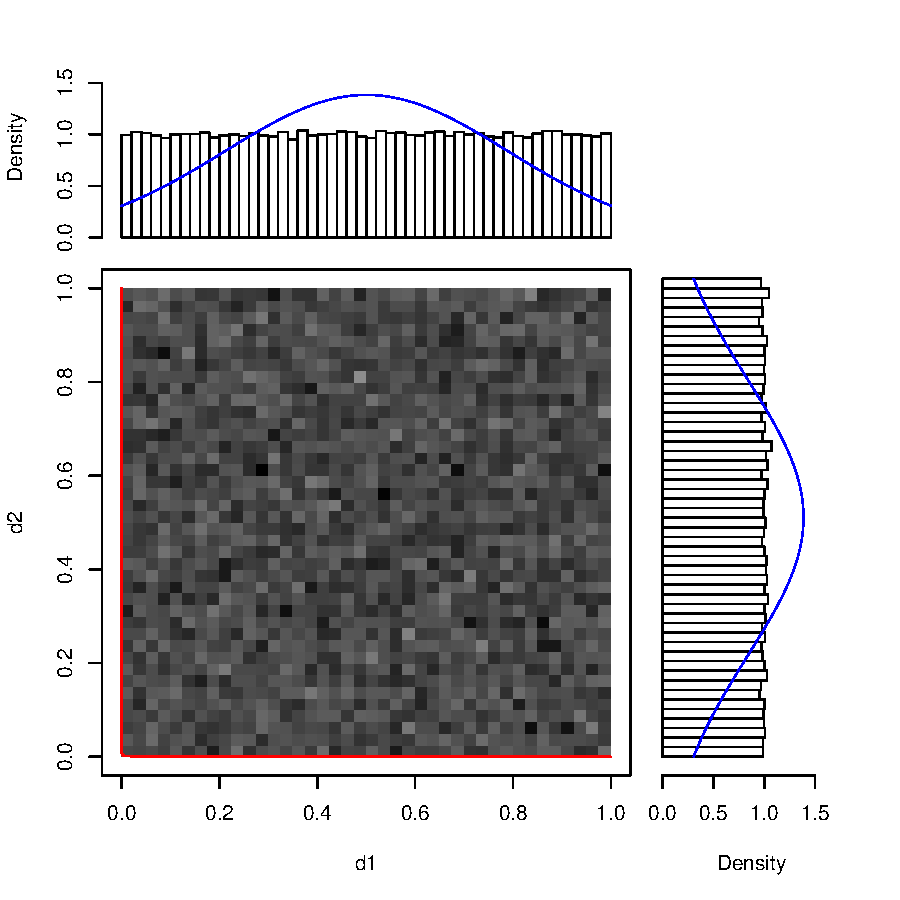
\includegraphics[width=100mm]{plots/density-2d-i2d1e5}
\caption{Density plot for independent dataset (100k tuples)}
\label{fig:density-2d-i2d1e5}
\end{figure}

\item \emph{corr}: 
a correlated dataset represents an environment in which points which
are good in one dimension are also good in the other dimensions. 

%For instance, students which have a good publication record typically also
%do well in their preliminaries. 

A vextor $x$ with the dimension $dim$ is generated in the following way:

\begin{lstlisting}
do
{
	int	d;
	double	v = random_peak(0, 1, dim);
	double	l = v <= 0.5 ? v : 1.0 - v;
	
	for (d = 0; d < dim; d++)
		x[d] = v;

	for (d = 0; d < dim; d++)
	{
		double h = random_normal(0, l);
		x[d] += h;
		x[(d + 1) % dim] -= h;
	}
} while (!is_vector_ok(dim, x));
\end{lstlisting}

Due to the way it is computed, \texttt{is\_vector\_ok()} ensures that all
coordinates of $x$ are within the interval $[0,1]$.

Figure \ref{fig:density-2d-c2d1e5} shows a correlated
dataset with 100k tuples for $d = 2$.

\begin{figure}[htbp]
\centering
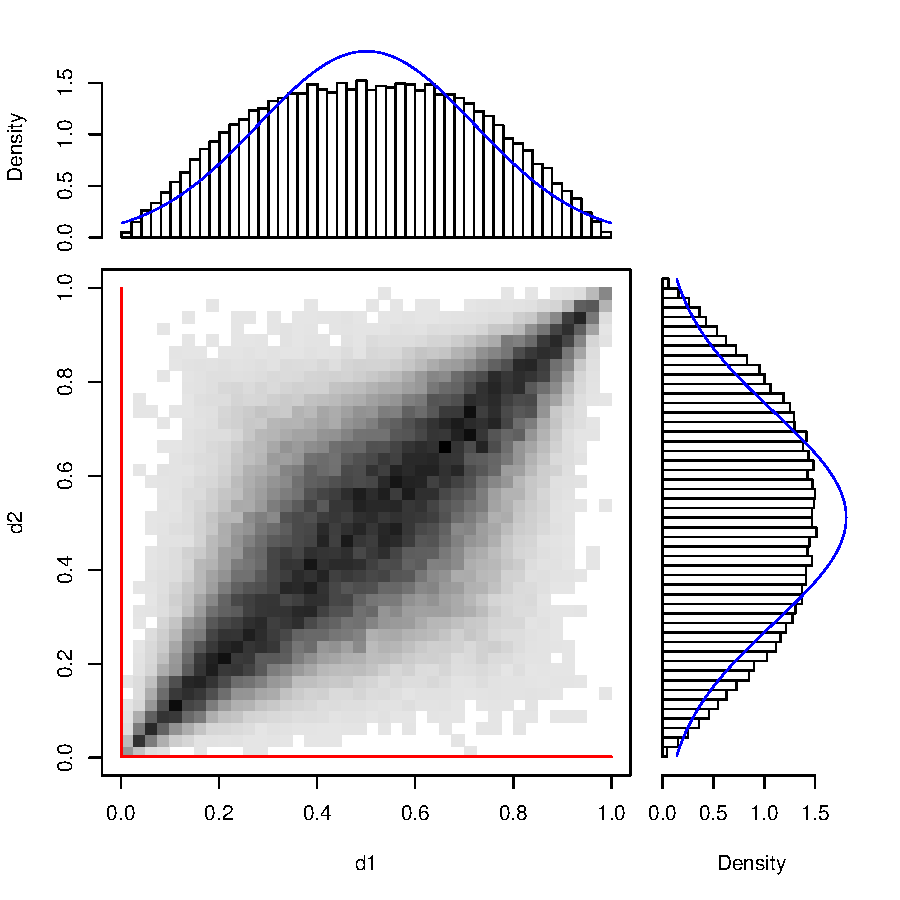
\includegraphics[width=100mm]{plots/density-2d-c2d1e5}
\caption{Density plot for correlated dataset (100k tuples)}
\label{fig:density-2d-c2d1e5}
\end{figure}


\item \emph{anti}:
an anti-correlated database represents an environment in which points
which are good in one dimension are bad in one or all of the other
dimensions; hotels seem to fall into this category. As for a
correlated database, we generate a point by first selecting a plane
perpendicular to the line from (0, . . . , 0) to (1, . . . , 1) using
a normal distribution. We use a normal distribution with very small
variance so that all points are placed into planes which are close to
the plane through the point (0.5, . . . , 0.5).  Within the plane, the
individual attribute values are generated using a uniform
distribution. Figure
\ref{fig:density-2d-a2d1e5} shows an anti-correlated dataset with 100k
tuples for $d = 2$.
\end{itemize}

\begin{figure}[htbp]
\centering
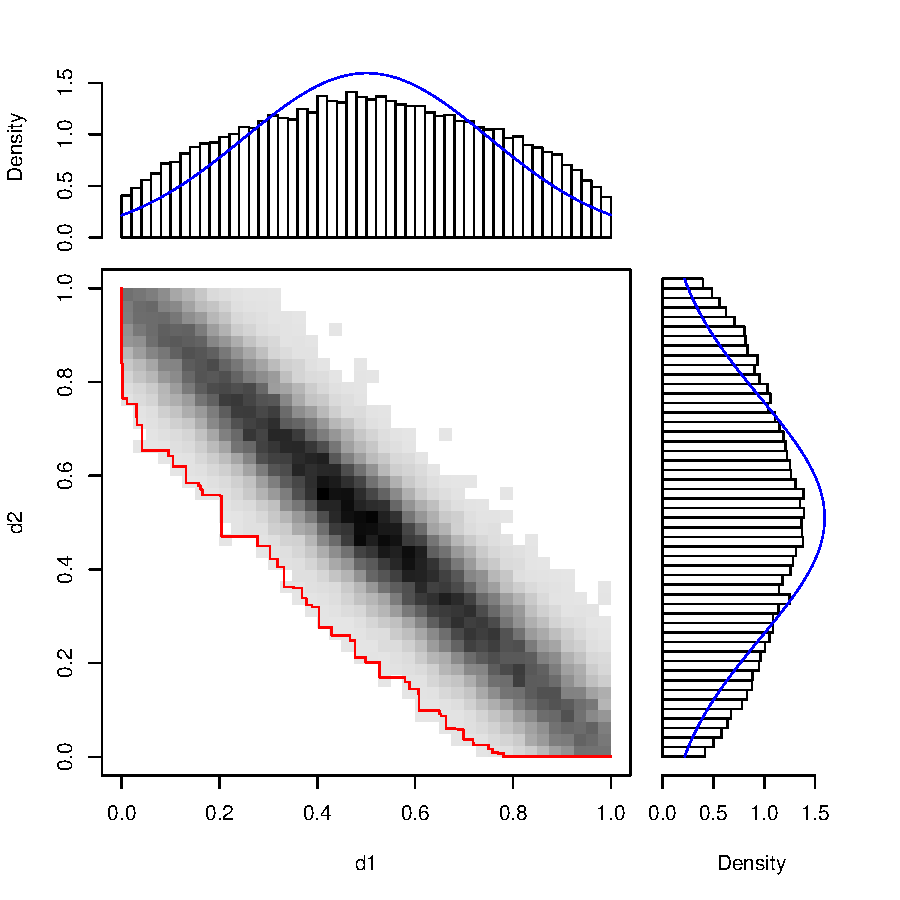
\includegraphics[width=100mm]{plots/density-2d-a2d1e5}
\caption{Density plot for anti-correlated dataset (100k tuples)}
\label{fig:density-2d-a2d1e5}
\end{figure}

For the very details of the random dataset generator, please have a
look at the implementation which is available at \citep{Eder2007a}.

\subsubsection{As command line utility}

The usage message explains, how to use the command line utility
\begin{shellscript}
\cmd{randdataset -?}

Test Data Generator for Skyline Operator Evaluation
Usage: randdataset (-i|-c|-a) -d DIM -n COUNT [-s SEED] [-p] [-S] [-h|-?]

Options:
       -i       independent (dim >= 1)
       -c       correlated (dim >= 2)
       -a       anti-correlated (dim >= 2)

       -d DIM   dimensions >=1
       -n COUNT number of vectors
       -I       unique id for every vector
       -p PAD   add a padding field, PAD characters long

       -C       generate SQL COPY statement
       -R       generate SQL CREATE TABLE statement
       -T NAME  use NAME instead of default table name

       -s SEED  set random generator seed to SEED

       -S       output stats to stderr

       -h -?    display this help message and exit

Examples:
       randdataset -i -d 3 -n 10 -I -R
       randdataset -a -d 2 -n 100 -S
\end{shellscript}

An invocation of \texttt{randdataset} suitable to pipe it directly into \texttt{psql}, i.e. load it into database, could look like: 

\begin{shellscript}
\cmd{randdataset -i -d 3 -n 10 -I -R}

DROP TABLE IF EXISTS "i3d10";
CREATE TABLE "i3d10" (id int, d1 float, d2 float, d3 float);
COPY "i3d10" (id, d1, d2, d3) FROM STDIN DELIMITERS ',' CSV QUOTE '''';
1,0.000000000000000e+00,6.900010321708401e-01,5.054183972559023e-01
2,5.914905399975788e-01,5.547849133400177e-01,3.784288188342139e-01
...
10,8.585111004572880e-01,9.898449857671955e-02,8.770675234855467e-01
\ttbackslash.
\end{shellscript}

\subsubsection{PostgreSQL Random Dataset Generator Function}

To test drive this PostgreSQL 'contrib' module (see
\srcref(contrib/randdataset)), without installing it, even with
installing PostgreSQL visit our webinterface at
\url{http://skyline.dbai.tuwien.ac.at/}. To install it onto your
PostgreSQL installation follow the instructions
\srcref{contrib/randdataset/README.randdataset}. Once installed the
function can be used as follows:

\begin{verbatim}
select * from
pg_rand_dataset('indep', 2, 10, 0) ds(id int, d1 float, d2 float);

select * from
pg_rand_dataset('corr', 3, 10, 0) ds(id int, d1 float, d2 float, d3 float);

select * from
pg_rand_dataset('anti', 3, 20, 0) ds(id int, d1 float, d2 float, d3 float);
\end{verbatim}

The general signatur for \inlinesql{pg\_rand\_dataset} is:
\begin{verbatim}
FUNCTION pg_rand_dataset(disttype text, dim int, rows int, seed int)
RETURNS setof record
\end{verbatim}

Where the arguments have following meaning:
\begin{itemize}
\item \texttt{disttype} specifies the distribution type (see section \ref{sec:corr-anti-indep}), allowed values are \texttt{'indep'}, \texttt{'corr'}, and \texttt{'anti'}

\item \texttt{dim} specifies the number of dimensions, allowed values are 1 upto 20 

\item \texttt{rows} specifies the number of tuples that should be returned, and 

\item \texttt{seed} is the seed for the random generator
\end{itemize}

We ensured that calling \inlinesql{pg\_rand\_dataset} with the same
arguments will always return the same result set. In the PostgreSQL
terminology this property of a function is called \texttt{IMMUTABLE}
(see PostgreSQL documentation on
\postgresdocu{xfunc-volatility.html}{Function Volatility Categories}).

To make the usage more comfortable we defined a set of wrapper
functions \texttt{rds$k$d} for the dimenions $k \in \{1, \ldots,
20\}$, they allowed us to issue the same queries as above in the
following why (see \srcref{contrib/randdataset/randdataset.sql.in}):

\begin{verbatim}
select * from rds2d('indep', 10, 0);

select * from rds3d('corr', 10, 0);

select * from rds3d('anti', 20, 0);
\end{verbatim}


\subsubsection{Buffer for Set returning function}
we patched PostgreSQL, to avoid swapping of our intermediate result to disk

\todo{}{append patch here? why not it's short}
% function_scan_work_mem.diff

\subsubsection{more stuff}
N(0,1) in kossmann generator.txt

http://de.wikipedia.org/wiki/Normalverteilung\#Box-Muller-Methode

die zw�lfer regel scheint problematisch,

ein mal spektrum analysieren

ev. erf verwenden \#include <math.h>




\subsection{window size}
assumtions on windowsize:

the assumtion that at no time more than output\_tuples will be in the window can not be hold.

larger window and and less passes do not always mean better runtime

infact there is a break even point


\clearpage % \todo{remove clearpage}{}

\section{Benchmarking}
\todo{see \citep{Gray1993}}{}

There is a large number of parameters that can be varied:

\begin{itemize}
\item \emph{size of dataset} (100?, 1000?, 10000, 100000, 1000000)
\item \emph{number of dimensions} (1-15, or even 10 is enough)
\item \emph{data distribution} (indep, corr, anti)
\item \emph{data source} (disk, set returning function)

in case the data are stored on disk
\begin{itemize}
\item \emph{sequencial scan vs. index scan} SFS can benefit from index scan (ommit sort phase), BNL and SFS could benefit from a index scan if DIFF groups are used.
\item \emph{sequence of tuples in tuple stream} (random, high entropy first/last) for BNL and EF if a very good tuple is very early in the tuple stream it will eliminate a lot of tuples in a very early stage
\end{itemize}
\item \emph{methods}

\begin{itemize}
\item as SQL statement
\item special case 1 dim distinct
\item special case 1 dim 
\item special case 2 dim (needs sort presort or access path)
\item BNL
\item SFS
\item EF+SFS=LESS
\item EF+BNL
\end{itemize}

\item window size
\item window policy (prepend, append, entropy)
\item entropy needs stats for scaling to (0,1)

\end{itemize}

Todo's

\begin{itemize}
\item use 90\% percentile (\citep{Gray1993}[page 315]) vs, average / variance (box-plots?)
\item describe software (operating system: Windows XP + SP 2, Microsoft Visual Studio 2005 + SP1, based on PostgreSQL 8.3.0) and hardware (CPU, RAM, Disk config, File System) used for benchmarking

\item describe the configuration of PostgreSQL (flags used for \texttt{configure --enable-asserts --enable-checks, ...}, it is recommended to turn asserts and co. off for benchmarking

\item \todo{maybe run all the tests on dmdb2.bda.local = Dell OptiPlex XXX, to have a off the shelf hardware}{}
\end{itemize}



\chapter*{Summary\revision}
\section{Futher work}

use special algorithms if we deal with domains with small cardinalites, \citep{Preisinger2006, Preisinger2007, Morse2007}

use seperate windows for each skyline group? or use hashing to reduce the number of comparisons?

hashing seams to be promissing for skyline groups.

implement $K$-skyband (maintaine dominance count in tuple window) do so for BNL and SFS.




\addcontentsline{toc}{chapter}{Summary\revision}



